\begin{table*}\centering
\ra{1.3}
\begin{tabular}{@{}ccccc@{}}\toprule
 \multicolumn{2}{c}{\textbf{Distribution A}} &&  \multicolumn{2}{c}{\textbf{Distribution B}} \\ 
 \cmidrule{1-2} \cmidrule{4-5}
Positives& Negatives & \phantom{ab} & Positives & Negatives\\
    \begin{minipage}{.2\textwidth}
      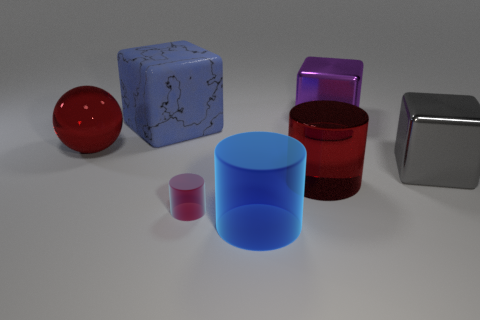
\includegraphics[width=\linewidth]{figures/clevr_datasets/CLEVRA_examples/train1.png}
    \end{minipage}
    &
    \begin{minipage}{.2\textwidth}
      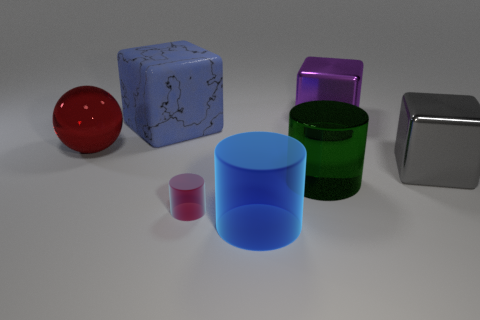
\includegraphics[width=\linewidth]{figures/clevr_datasets/CLEVRA_examples/train_color1.png}
    \end{minipage}
    &&
    \begin{minipage}{.2\textwidth}
      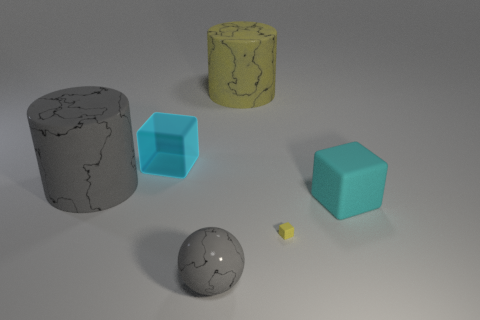
\includegraphics[width=\linewidth]{figures/clevr_datasets/CLEVRA_examples/test1.png}
    \end{minipage}
    &
        \begin{minipage}{.2\textwidth}
      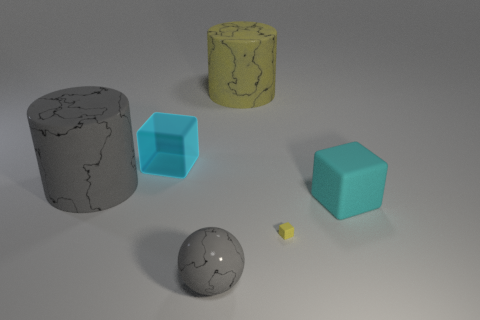
\includegraphics[width=\linewidth]{figures/clevr_datasets/CLEVRA_examples/test_color1.png}
    \end{minipage}
\\ \\
    \begin{minipage}{.2\textwidth}
      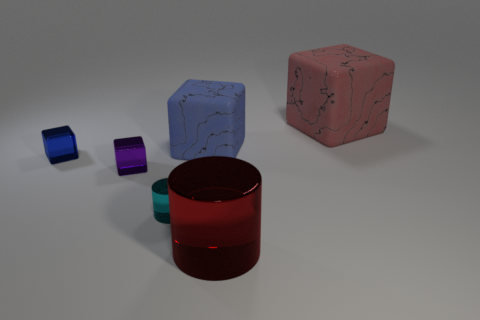
\includegraphics[width=\linewidth]{figures/clevr_datasets/CLEVRA_examples/train2.png}
    \end{minipage}
    &
    \begin{minipage}{.2\textwidth}
      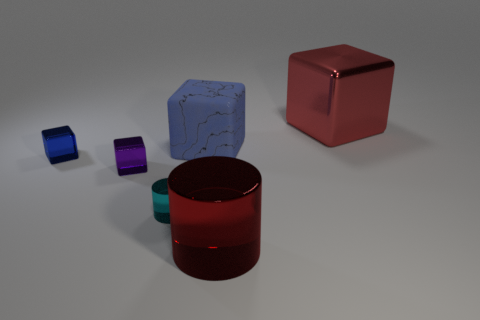
\includegraphics[width=\linewidth]{figures/clevr_datasets/CLEVRA_examples/train_material2.png}
    \end{minipage}
    &&
    \begin{minipage}{.2\textwidth}
      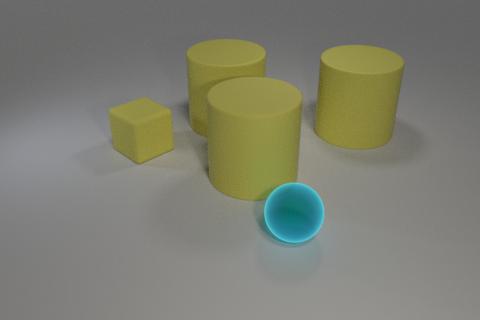
\includegraphics[width=\linewidth]{figures/clevr_datasets/CLEVRA_examples/test2.png}
    \end{minipage}
    &
        \begin{minipage}{.2\textwidth}
      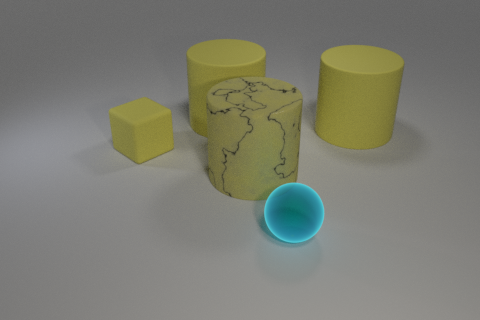
\includegraphics[width=\linewidth]{figures/clevr_datasets/CLEVRA_examples/test_material2.png}
    \end{minipage}
\\ \\
    \begin{minipage}{.2\textwidth}
      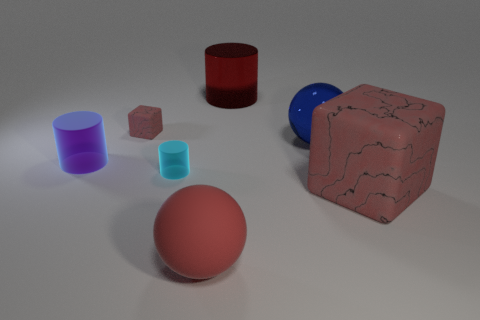
\includegraphics[width=\linewidth]{figures/clevr_datasets/CLEVRA_examples/train3.png}
    \end{minipage}
    &
    \begin{minipage}{.2\textwidth}
      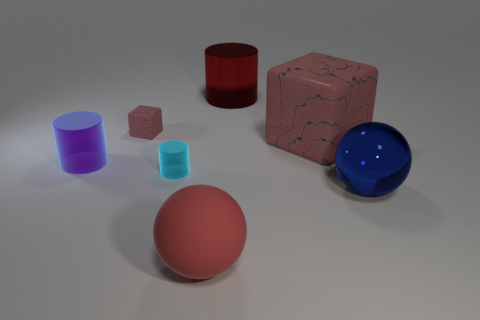
\includegraphics[width=\linewidth]{figures/clevr_datasets/CLEVRA_examples/train_relation3.png}
    \end{minipage}
    &&
    \begin{minipage}{.2\textwidth}
      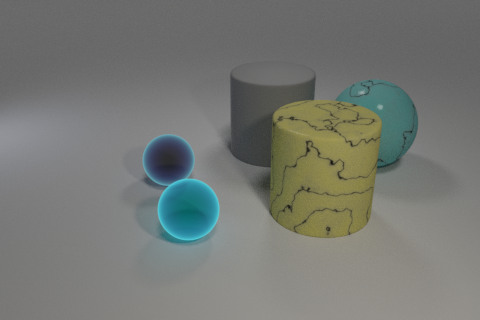
\includegraphics[width=\linewidth]{figures/clevr_datasets/CLEVRA_examples/test3.png}
    \end{minipage}
    &
        \begin{minipage}{.2\textwidth}
      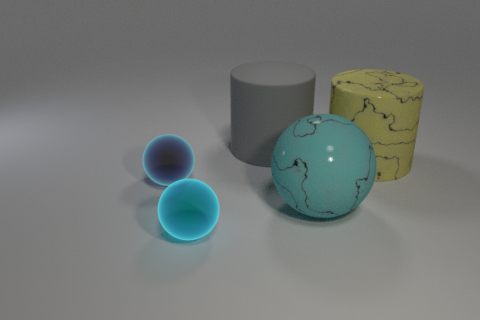
\includegraphics[width=\linewidth]{figures/clevr_datasets/CLEVRA_examples/test_relation3.png}
    \end{minipage}
\\ \\
    \begin{minipage}{.2\textwidth}
      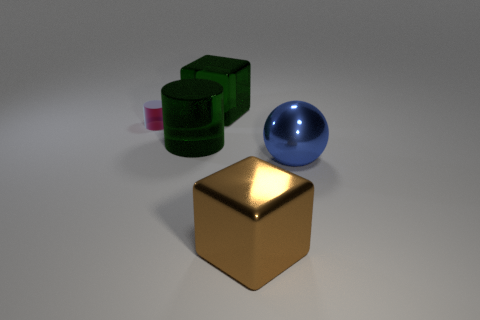
\includegraphics[width=\linewidth]{figures/clevr_datasets/CLEVRA_examples/train4.png}
    \end{minipage}
    &
    \begin{minipage}{.2\textwidth}
      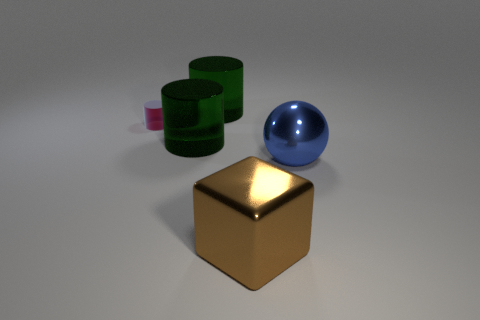
\includegraphics[width=\linewidth]{figures/clevr_datasets/CLEVRA_examples/train_shape4.png}
    \end{minipage}
    &&
    \begin{minipage}{.2\textwidth}
      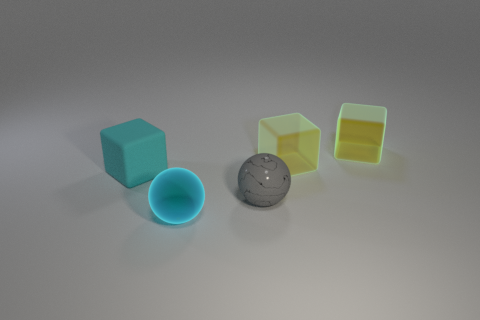
\includegraphics[width=\linewidth]{figures/clevr_datasets/CLEVRA_examples/test4.png}
    \end{minipage}
    &
        \begin{minipage}{.2\textwidth}
      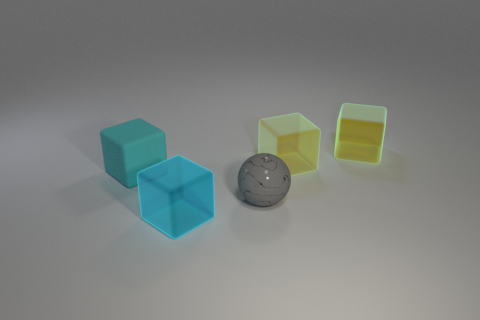
\includegraphics[width=\linewidth]{figures/clevr_datasets/CLEVRA_examples/test_shape4.png}
    \end{minipage}
\\ \\
    \begin{minipage}{.2\textwidth}
      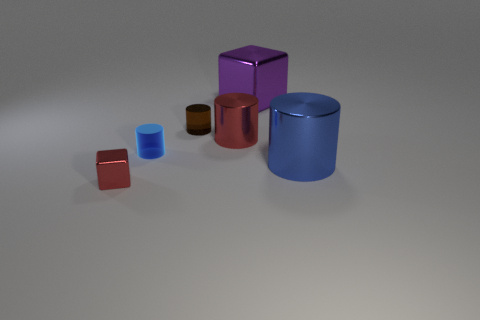
\includegraphics[width=\linewidth]{figures/clevr_datasets/CLEVRA_examples/train5.png}
    \end{minipage}
    &
    \begin{minipage}{.2\textwidth}
      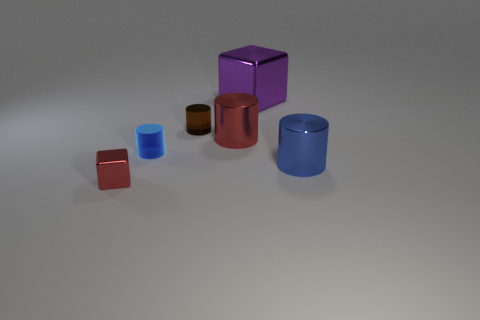
\includegraphics[width=\linewidth]{figures/clevr_datasets/CLEVRA_examples/train_size5.png}
    \end{minipage}
    &&
    \begin{minipage}{.2\textwidth}
      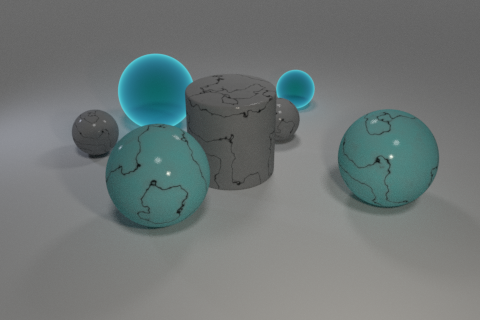
\includegraphics[width=\linewidth]{figures/clevr_datasets/CLEVRA_examples/test5.png}
    \end{minipage}
    &
        \begin{minipage}{.2\textwidth}
      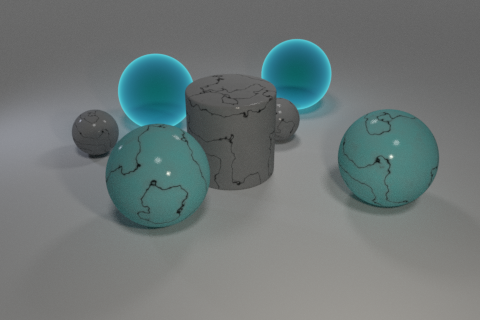
\includegraphics[width=\linewidth]{figures/clevr_datasets/CLEVRA_examples/test_size5.png}
    \end{minipage}
\\ 

\bottomrule
\end{tabular}
\caption[CLEVR\_B dataset examples]{CLEVR\_B dataset examples. There are five examples from each distribution, with corresponding negatives. Each row shows a different negative (color, material, relation, shape, size). There is a negative for each attribute and each image, so there are a total of six similar images for each example (positive and five negatives), though in this table we only show the positive and one of the negatives.}
\end{table*}